\section{Model Choice and Hyperparameters}
% How you are determining what model(s) to use in your final pred.py, as well as an exploration of hyperparameters. We are looking for:
% – A convincing explanation of how you ensured that the evaluation metrics for various models are comparable (i.e., are you using a consistent test set?)
% – A clear description of the evaluation metric(s) used to evaluate your model, as well as justification for its use.
% – A description of the hyperparameters that you are tuning, hyperparameter value combinations that you have tried, and the value of the evaluation metric(s) for those hyperparameters. We are not looking for an exhaustive search of all possible hyperparameter combinations, but there should be enough evidence to demonstrate that your hyperparameter choices are reasonable. (Note that just saying “X was the best hyperparameter value based on metric Y out of the hyperparameter values we tried” is not enough. Please present the values of the evaluation metrics for each hyperparameter value to show that your choice was the best one.)
% – A clear description of what your final model choice looks like in the submitted pred.py file.
% – The descriptions should be consistent with the .py and/or .ipynb files that you used while developing your model.

\subsection{Word Embedding - Neural Network}
\begin{table}[h]
    \centering
    \begin{tabular}{lccc}
        \hline
        Category     & Precision                              & Recall & F1-score \\
        \hline
        Pizza        & 0.82                                   & 0.83   & 0.83     \\
        Shawarma     & 0.91                                   & 0.82   & 0.86     \\
        Sushi        & 0.78                                   & 0.88   & 0.83     \\
        \hline
        Accuracy     & \multicolumn{3}{c}{0.84 (329 samples)}                     \\
        Macro avg    & 0.84                                   & 0.84   & 0.84     \\
        Weighted avg & 0.84                                   & 0.84   & 0.84     \\
        \hline
    \end{tabular}
    \caption{Classification Report}
\end{table}
\begin{table}[h]
    \centering
    \begin{tabular}{ccc}
        \hline
        Loss   & Bias   & Variance \\
        \hline
        0.2345 & 0.2345 & 0.0149   \\
        \hline
    \end{tabular}
\end{table}

\begin{figure}[h]
    \centering
    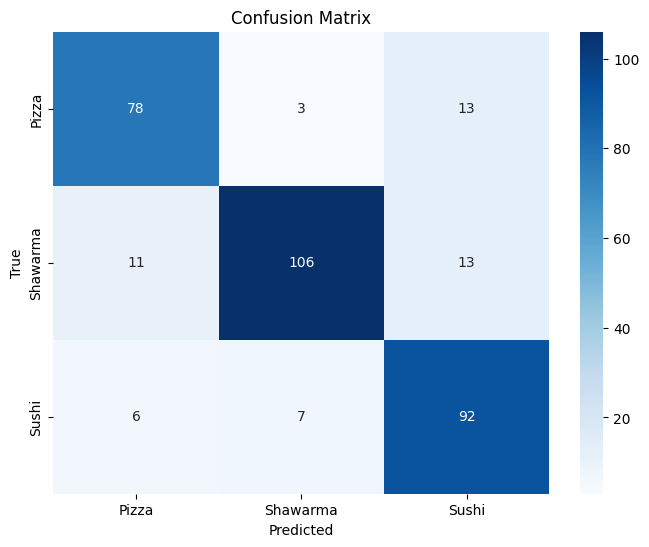
\includegraphics[width=0.45\textwidth]{params/neuralnetwork_confusion.png}
    \caption{Confusion Matrix for Neural Network}
\end{figure}

\subsection{Word Embedding - Linear Regression}
\begin{table}[h]
    \centering
    \begin{tabular}{lccc}
        \hline
        Category     & Precision                              & Recall & F1-score \\
        \hline
        Pizza        & 0.81                                   & 0.90   & 0.85     \\
        Shawarma     & 0.91                                   & 0.84   & 0.87     \\
        Sushi        & 0.87                                   & 0.86   & 0.86     \\
        \hline
        Accuracy     & \multicolumn{3}{c}{0.86 (329 samples)}                     \\
        Macro avg    & 0.86                                   & 0.87   & 0.86     \\
        Weighted avg & 0.87                                   & 0.86   & 0.86     \\
        \hline
    \end{tabular}
    \caption{Classification Report}
\end{table}

\begin{table}[h]
    \centering
    \begin{tabular}{ccc}
        \hline
        Loss   & Bias   & Variance \\
        \hline
        0.2518 & 0.2518 & 0.0091   \\
        \hline
    \end{tabular}
\end{table}

\begin{figure}[h]
    \centering
    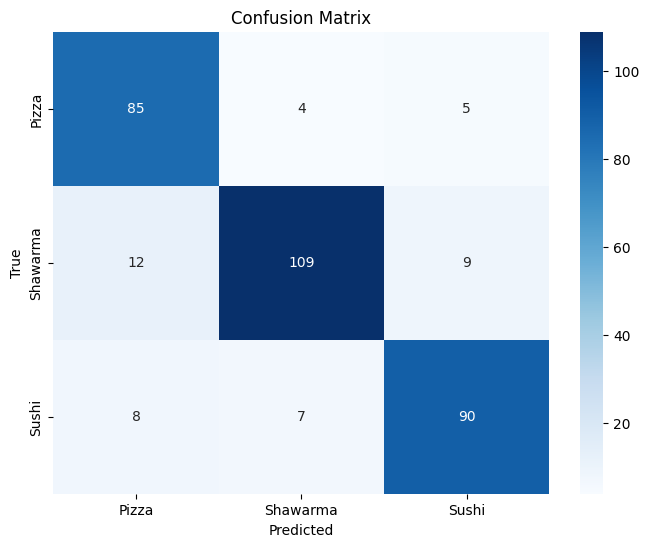
\includegraphics[width=0.45\textwidth]{params/linearregression_confusion.png}
    \caption{Confusion Matrix for Linear Regression}
\end{figure}